\section{Technologies}
Here we will examine the complete technologies of the tablet.

\begin{wrapfigure}{R}{0.3\textwidth}
\centering
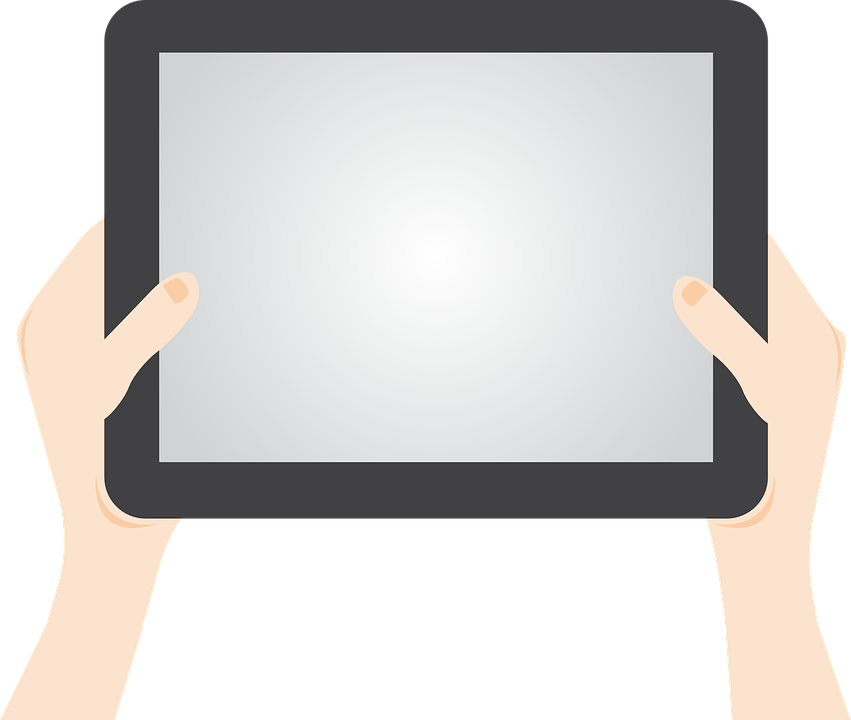
\includegraphics[width=0.3\textwidth, keepaspectratio]{images/pact/tablet}
\caption{\label{fig:technologies}Picture of a tablet, which might run the application.}
\end{wrapfigure}
\begin{itemize}[noitemsep]
    \item Bluetooth capabilities
    \item Wireless internet 
    \item Camera
    \item GPS
    \item Timer 
    \item Clock 
    \item Flashlight 
    \item Storage of digital information 
    \item Loudspeakers 
    \item Touchscreen
    \item Digital games 
    \item Personal assistant (digital)
    \item Accelerometer
    \item GSM, HDSPA, LTE (cellular network)
    \item NFC (near field communication)
\end{itemize}

\subsection{Input}
The input of the tablet is primarily its touchscreen and the physical buttons placed on the device such as the on/off button or the volume. Secondary the input of the tablet is the voice controlled command the newer models supports. Some model of the tablet also have a small keyboard for input.

\subsection{Output}
The output of the average tablet is the tablets display/screen where it is possible for the tablet to show the user a wide array of different information. The output would also be sound as all tablets have a set of loudspeakers embedded in them or, at the very least, an audio jack. Sound could fx be used for encouragement for the user to pay attention to the device. 

\subsection{Communication}
The possibilities of communication in a tablet is Wi-Fi, Bluetooth, mobile data connection and NFC. These can be used to communicate data to an offsite server or communicate with other users. The GPS can be used to communicate the location of the user or equipment to a tracking system.
